% WBC-MJLab Technical Report (arXiv draft)
% Build: pdflatex main && bibtex main && pdflatex main && pdflatex main
% Or: latexmk -pdf main.tex
\documentclass[11pt,a4paper]{article}

\usepackage[margin=1in]{geometry}
\usepackage[T1]{fontenc}
\usepackage{lmodern}
\usepackage{microtype}
\usepackage{amsmath,amssymb}
\usepackage{booktabs}
\usepackage{tabularx}
\usepackage{graphicx}
\usepackage{xcolor}
\usepackage{hyperref}
\usepackage{url}
\usepackage{enumitem}
\usepackage{tikz}
\usetikzlibrary{arrows.meta,positioning,fit,calc}
\usepackage[numbers,sort&compress]{natbib}
\usepackage{fancyhdr}
\usepackage{titlesec}
\usepackage{listings}
\usepackage{caption}
\usepackage[nameinlink,noabbrev]{cleveref}
\usepackage{placeins}

\newcommand{\LiveDemoURL}{https://wbc-mjlab.github.io/wbc-demo/}

\hypersetup{
  colorlinks=true,
  linkcolor=black,
  citecolor=blue!50!black,
  urlcolor=blue!50!black,
}

\lstset{
  basicstyle=\ttfamily\footnotesize,
  columns=fullflexible,
  keepspaces=true,
  frame=single,
  framesep=4pt,
  xleftmargin=2pt,
  xrightmargin=2pt,
  aboveskip=0.6em,
  belowskip=0.6em,
  breaklines=true,
  breakatwhitespace=true,
}

\setlength{\headheight}{14pt}
\pagestyle{fancy}
\fancyhf{}
\fancyhead[L]{\textsc{wbc-mjlab}}
\fancyhead[R]{Technical Report · v0.0.6}
\fancyfoot[C]{\thepage}
\renewcommand{\headrulewidth}{0.4pt}

\titleformat{\section}{\large\bfseries}{\thesection}{0.6em}{}
\titleformat{\subsection}{\normalsize\bfseries}{\thesubsection}{0.5em}{}

\title{%
  \vspace{-1.5em}
  {\LARGE\bfseries wbc-mjlab}\\[0.4em]
  {\large Unified Whole-Body Motion Tracking on mjlab}\\[0.6em]
  {\normalsize\url{https://github.com/wbc-mjlab/wbc-mjlab}}
}

\author{%
  Simeon Nedelchev$^{1,2}$ \hspace{1.4em}
  Anton Chaplygin$^{3}$ \hspace{1.4em}
  Lev Kozlov$^{4}$ \\[0.35em]
  Ivan Domrachev$^{4}$ \hspace{1.4em}
  Ekaterina Chaikovskaia$^{1}$ \\[0.8em]
  $^{1}$Institute of Artificial Intelligence, MIPT \quad
  $^{2}$Innopolis University \\
  $^{3}$Robotics Center SBER \\
  $^{4}$KAIST
}

\date{}

\begin{document}
\maketitle
\thispagestyle{fancy}
\vspace{-1.4em}

\noindent
\href{\LiveDemoURL}{%
  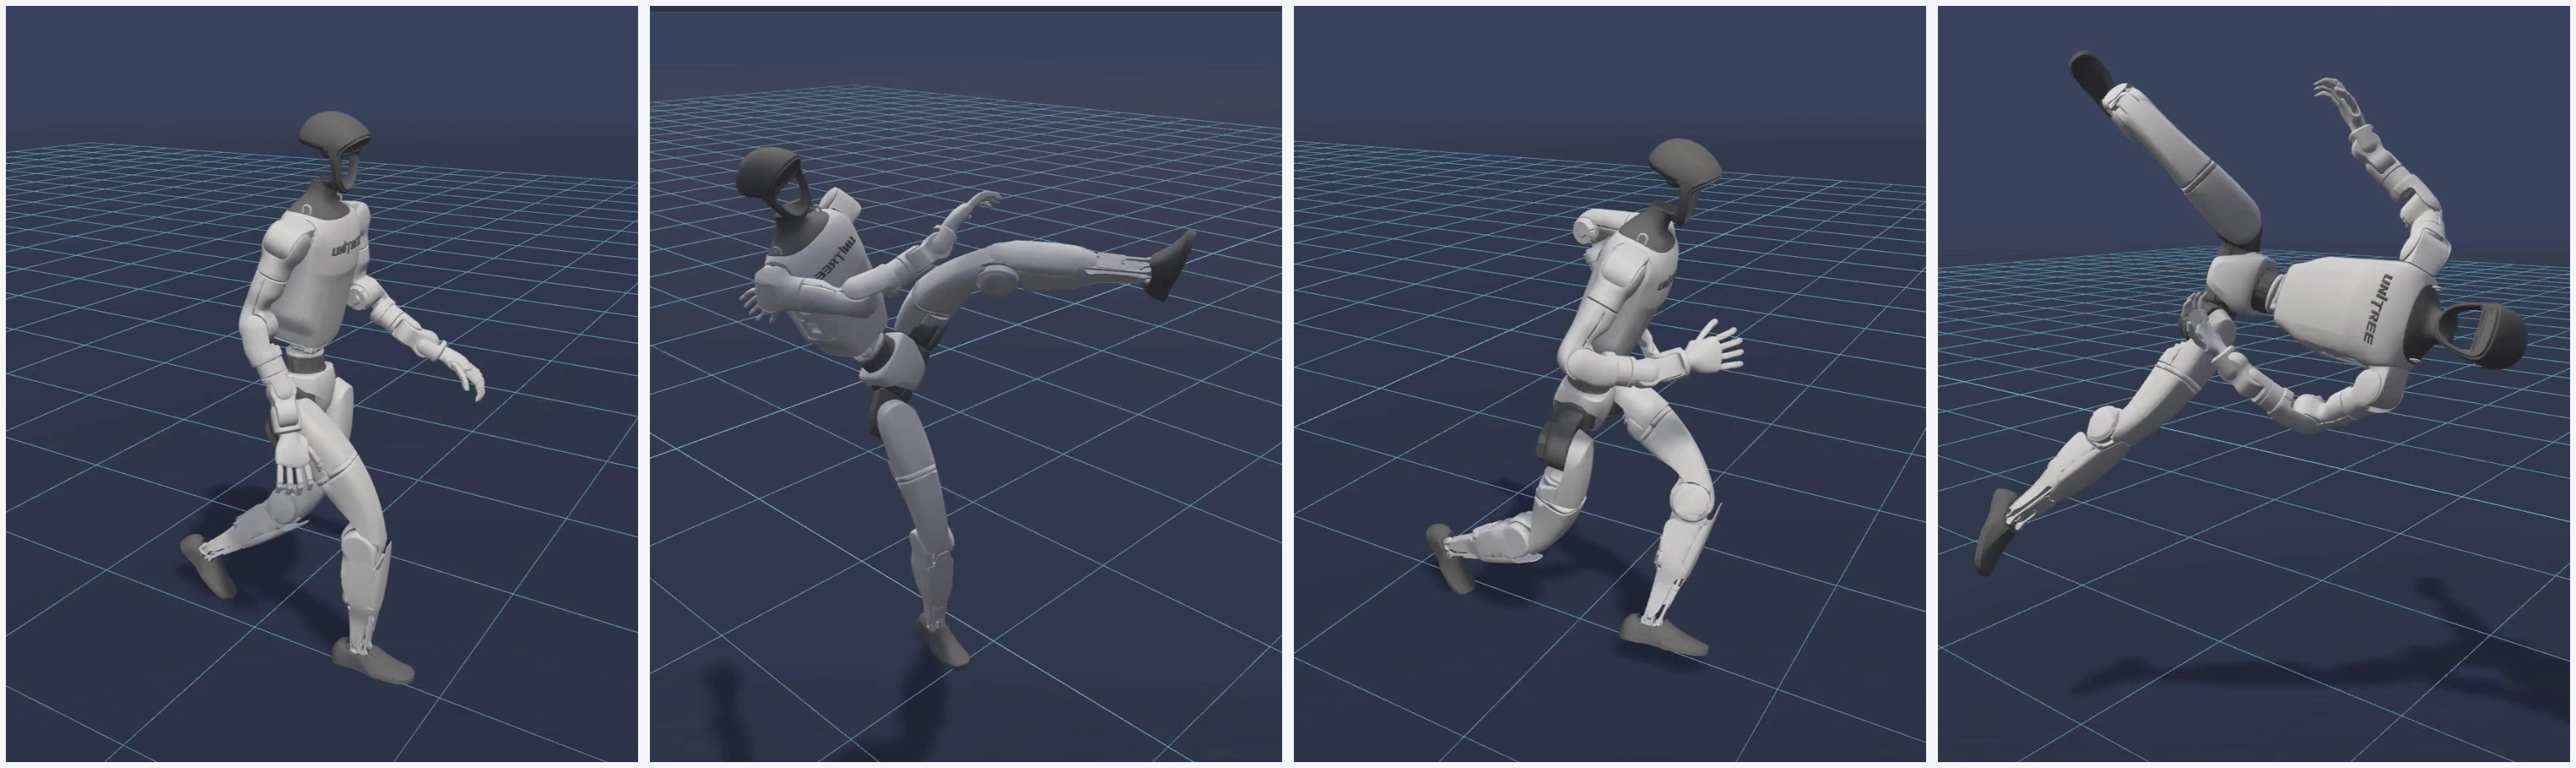
\includegraphics[width=\textwidth]{figures/collage.jpg}%
}
\vspace{0.35em}
\captionsetup{type=figure, font=small, justification=centering, skip=6pt}
\caption*{Unitree G1 whole-body motion tracking on a multi-clip library
(\emph{left to right}: walk, kick, run, side flip). \textbf{Click the collage} to
open the live browser demo
(\href{\LiveDemoURL}{\nolinkurl{\LiveDemoURL}}).}
\vspace{0.4em}

\begin{abstract}
\noindent
We present \textsc{wbc-mjlab}, an open-source training
library for whole-body motion tracking on mjlab~\citep{zakka2026mjlab}. The
library factors the low-level tracker shared by recent humanoid systems into
one manager-based MDP: scaled residual joint actions, a multi-clip motion
command with adaptive reference-state initialization (RSI), exponential
tracking rewards on anchor and keybody kinematics, and a composable catalog of
motion-reference observations. Paper-specific choices---ZEST-style end-effector
tracking and assistive wrench~\citep{zest2026}, BeyondMimic-style binary-failure
RSI~\citep{liao2025beyondmimic}, state-estimation actor layouts, per-channel
observation noise---are expressed as \emph{presets} on the same template rather
than separate codebases. Robots plug in as entities; training emits exported
artifacts that downstream runtimes can consume for modular deploy. The goal is a
comparable, robot-agnostic surface for multi-skill
control on MuJoCo Warp~\citep{mujoco_warp2025}.
\end{abstract}

% ===========================================================================
\section{Introduction}
% ===========================================================================

Humanoid whole-body control increasingly relies on reinforcement learning from
motion libraries: a policy tracks reference kinematics in simulation and
transfers to hardware. Recent systems converge on the same low-level
recipe---exponential tracking rewards, adaptive reference-state initialization
(RSI), and residual joint actions---while differing in higher-level goals such
as skill composition~\citep{liao2025beyondmimic}, zero-shot
transfer~\citep{zest2026}, or foundation-scale
training~\citep{sonic2025,omnixtreme2026}. Despite that overlap, each line of
work tends to ship as its own codebase, so comparing a single design choice or
porting a recipe to a new robot means navigating divergent APIs.

\textsc{wbc-mjlab} is a training library on mjlab~\citep{zakka2026mjlab}
(MuJoCo Warp~\citep{mujoco_warp2025}, Isaac Lab's manager-based
API~\citep{mittal2025isaaclab}, RSL-RL~\citep{schwarke2025rslrl}). It does not
introduce a new control method; it factors the shared tracker into one MDP and
treats paper- and deploy-specific choices as configuration. Relative to monolithic
Isaac Lab stacks~\citep{hybridrobotics_wbt,nvlabs_groot_wbc2026},
\textsc{wbc-mjlab} targets a smaller, robot-agnostic training surface: one
motion command feeds all tracking terms and actor layouts are assembled from a
reference catalog.

\paragraph{Contributions.}
\begin{enumerate}[leftmargin=1.4em,itemsep=0.25em]
  \item A \textbf{shared tracker MDP} with explicit reward and RSI mathematics:
        scaled residual actions, anchor-relative keybody tracking, exponential
        kernels with ZEST-compatible sharpness~\citep{zest2026}, reward-aligned
        adaptive RSI, terminations, and bin-coupled assistive wrench.
  \item \textbf{Presets and tasks}: pure configuration recipes (weights, body
        subsets, RSI strategy, observation layout) registered per robot without
        forking the MDP; extension packages add platforms.
  \item A \textbf{train-to-deploy path}: motion libraries $\to$ training
        $\to$ exported policy artifacts usable by modular deploy runtimes.
\end{enumerate}

\paragraph{Design commitments.}
Four principles decide what belongs in core code versus configuration.
(1)~Tracking callables live once in the MDP; a \emph{preset} only reweights or
toggles pre-populated slots.
(2)~A \emph{task} binds one robot entity to one preset stack so ablations are
task switches, not code branches.
(3)~Unitree G1 is the in-tree reference robot; other platforms ship as
\emph{extension packages} (Section~\ref{sec:extensions}) that plug into the
same MDP and presets.
(4)~Multi-clip libraries train one low-level tracker; at deploy time the
reference stream may come from clips, teleop, or a higher-level policy.
Planning UIs and hardware drivers stay outside this repository; physics and
optimization loops are upstream in mjlab and RSL-RL.

Sections~\ref{sec:architecture}--\ref{sec:workflows} describe architecture,
the shared MDP, presets, and the convert--train--export pipeline.
Section~\ref{sec:related} situates the library relative to prior systems.

% ===========================================================================
\section{Architecture}
\label{sec:architecture}
% ===========================================================================

\begin{figure}[t]
  \centering
  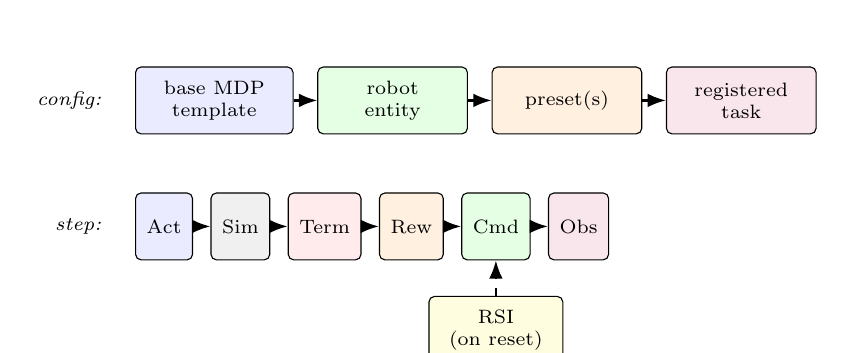
\begin{tikzpicture}[
    font=\scriptsize,
    box/.style={draw, rounded corners=2pt, align=center, inner sep=4pt,
      minimum height=0.85cm},
    arr/.style={-{Latex}, thick},
    dashedarr/.style={-{Latex}, thick, dashed},
    lbl/.style={font=\scriptsize\itshape, anchor=east},
  ]
    % --- config row ---
    \node[lbl] (config-lbl) at (0,0.45) {config:};
    \node[box, fill=blue!8, minimum width=2.0cm, right=0.3cm of config-lbl]
      (base) {base MDP\\template};
    \node[box, fill=green!10, right=0.3cm of base, minimum width=1.9cm] (robot)
      {robot\\entity};
    \node[box, fill=orange!12, right=0.3cm of robot, minimum width=1.9cm]
      (preset) {preset(s)};
    \node[box, fill=purple!10, right=0.3cm of preset, minimum width=1.9cm] (task)
      {registered\\task};
    \draw[arr] (base) -- (robot);
    \draw[arr] (robot) -- (preset);
    \draw[arr] (preset) -- (task);

    % --- step row ---
    \node[lbl] (step-lbl) at (0,-1.15) {step:};
    \node[box, fill=blue!8, right=0.3cm of step-lbl] (act) {Act};
    \node[box, fill=gray!12, right=0.22cm of act] (sim) {Sim};
    \node[box, fill=red!8, right=0.22cm of sim] (term) {Term};
    \node[box, fill=orange!12, right=0.22cm of term] (rew) {Rew};
    \node[box, fill=green!10, right=0.22cm of rew] (cmd) {Cmd};
    \node[box, fill=purple!10, right=0.22cm of cmd] (obs) {Obs};
    \draw[arr] (act) -- (sim);
    \draw[arr] (sim) -- (term);
    \draw[arr] (term) -- (rew);
    \draw[arr] (rew) -- (cmd);
    \draw[arr] (cmd) -- (obs);

    % RSI on reset (inside motion command)
    \node[box, fill=yellow!12, below=0.45cm of cmd, minimum width=1.7cm] (rsi)
      {RSI\\(on reset)};
    \draw[dashedarr] (rsi.north) -- (cmd.south);
  \end{tikzpicture}
  \vspace{0.4em}
  \caption{Configuration assembly (top) and mjlab per-step manager order
  (bottom). Adaptive RSI samples a reference frame on \emph{episode reset}
  inside the motion command, not between reward and observation each step.}
  \label{fig:architecture}
\end{figure}

Figure~\ref{fig:architecture} shows how configuration is composed and how a control
step is ordered. Every task builds a mjlab \texttt{ManagerBasedRlEnvCfg} by
layering four ingredients on a shared template:

\begin{enumerate}[leftmargin=1.4em,itemsep=0.15em]
  \item A base MDP template with all manager slots pre-populated (rewards,
        observations, terminations, events, RSI defaults).
  \item A robot entity: MuJoCo model, anchor body (torso or pelvis for global
        errors), keybody list, contact sensors, and per-joint action scales.
  \item One or more presets: reweight tracking terms, switch RSI strategy,
        edit the actor observation list, tighten terminations.
  \item Task registration: human-readable id, robot id, experiment name, and
        environment builder.
\end{enumerate}

At runtime a single \emph{motion command} advances the active clip, maintains
anchor-relative reference keybody poses, exposes reference kinematics to rewards
and observations, and may apply a bin-conditioned assistive wrench on the anchor.
On reset, adaptive RSI samples a (trajectory, temporal bin, frame), writes the
reference state into the simulator, and sets the episode assist gain (dashed path
in Figure~\ref{fig:architecture}). Each control step follows mjlab's manager order:
action, physics, termination, reward, command update, then observation.

\subsection{Library particularities}
\label{sec:particularities}
Several design choices distinguish this stack from a generic mjlab tracking
task~\citep{zakka2026mjlab} or monolithic Isaac Lab forks.

\paragraph{Single command, slot-based MDP.}
All tracking rewards, RSI statistics, reference observations, and assistive
wrench logic read one motion command instance. Parallel environments may track
different clips from the same NPZ library. Term callables are robot-agnostic:
body lists and weights come from configuration, not hard-coded skeletons.

\paragraph{Anchor-relative keybody targets.}
Style-critical body pose rewards compare the robot to reference keybodies in a
\emph{yaw-aligned anchor frame}: horizontal placement follows the robot anchor,
vertical height follows the reference anchor, and orientations are rotated by the
yaw delta between anchors (Section~\ref{sec:rewards}). Global root pose and twist
terms remain available for consistency. This split matches deploy practice where
global position drift is partially unobservable but relative limb pose is not.

\paragraph{Reward--RSI coupling.}
Adaptive RSI can score each simulation step either with hand-tuned exponential
kernels on joint and body errors, or---in the default WBC and ZEST presets---with
the \emph{same weighted sum of active tracking rewards} used for learning
(Section~\ref{sec:rsi}). Failure levels therefore rise where the policy actually
fails the training objective, not where a proxy metric disagrees.

\paragraph{Modular reference observations.}
Unlike mjlab's bundled \texttt{command} vector, reference kinematics are exposed
as independent observation terms (Section~\ref{sec:obs}). Presets drop, swap, or
reorder entries; each term may carry its own uniform noise. Playback, RSI, and
rewards stay unchanged---only the policy interface changes.

\paragraph{Train vs.\ play split.}
Play and evaluation disable observation corruption, motion domain randomization,
assistive wrench, and external pushes so in-sim rollouts match deploy. Training
keeps these aids active.

\paragraph{Preset composition.}
Presets are pure functions that mutate a shared config in place (no environment
fork). A state-estimation actor preset composes with any tracking preset by
replacing body height and reference gravity with pose-error terms while leaving reward
weights untouched.

% ===========================================================================
\section{Shared MDP}
\label{sec:mdp}
% ===========================================================================

Term callables take \texttt{command\_name}, body lists, and weights so they
stay robot-agnostic; presets only change configuration. Table~\ref{tab:mdp-glance}
groups the tracker into a control interface, a learning signal, and policy
inputs.

\begin{table}[t]
  \centering
  \small
  \caption{Shared MDP at a glance.}
  \label{tab:mdp-glance}
  \begin{tabular}{@{}lll@{}}
    \toprule
    Block & Component & Role \\
    \midrule
    Control & Action & scaled residual
      (Eq.~\eqref{eq:residual}) \\
     & Command & multi-clip playback, RSI, assist \\
    Learning & Reward & exponential tracking + regularizers \\
     & Reset / RSI & adaptive bin sampling \\
     & Terminations & early stops, moderate DR events \\
    Inputs & Observations & modular reference catalog \\
    \bottomrule
  \end{tabular}
\end{table}

\subsection{Control interface}
\label{sec:actions}
Under ZEST-style control~\citep{zest2026}, the default action outputs a residual
$a_t\in\mathbb{R}^{n_j}$ that is scaled and added to the motion command's
reference joints, then sent to joint PD:
\begin{equation}
  q^{\mathrm{des}}_t
    = q^{\mathrm{ref}}_t
      + s \odot a_t .
  \label{eq:residual}
\end{equation}
Here $q^{\mathrm{ref}}_t$ is the reference joint position at the current
command frame, $s\in\mathbb{R}^{n_j}_{>0}$ is a per-joint action scale, and
$\odot$ is elementwise multiplication. The policy commands a bounded correction
around the clip rather than absolute joint angles, which keeps the action
distribution stable across diverse motions.

The scale $s$ is configuration, not a learned parameter. The template defaults
to a uniform $s_j=0.25$. Robot entities override this with a per-DoF map
(e.g.\ G1 action scales), typically
\begin{equation}
  s_j = 0.25\,\frac{\tau^{\max}_j}{k_{p,j}},
  \label{eq:action-scale}
\end{equation}
where $\tau^{\max}_j$ is the actuator effort limit and $k_{p,j}$ the PD
stiffness. The ratio $\tau^{\max}/k_p$ is the steady-state position offset that
saturates the actuator under pure proportional control; the factor $0.25$ keeps
a unit-scale policy output inside a conservative fraction of that range.
Heterogeneous actuators (hips vs.\ wrists) therefore receive different residual
magnitudes automatically.

Absolute joint-position actions remain available for ablations, but force the
policy to rediscover the reference in action space. Unscaled residuals ($s=1$)
couple network outputs to joint range in a robot-specific way. Per-joint scales
tied to actuator limits travel with the robot entity, so the same preset stack
can run on different humanoids once each entity sets its own $s$.

The motion command supplies $q^{\mathrm{ref}}_t$ and all other reference
fields. It loads a multi-clip NPZ library (joint trajectories plus per-body
world-frame poses and velocities), advances kinematics each step, and drives
RSI at episode boundaries. Configuration includes the anchor body, keybody list,
pose and joint domain randomization at resample, RSI hyperparameters, and optional
assistive wrench. Rewards and reference observations bind to the command by name,
so a different playback source (clips, teleop, or planner) needs only a backend
that exposes the same kinematic fields.

\subsection{Learning signal}
\label{sec:rewards}
Tracking uses the exponential structure common to recent
systems~\citep{zest2026,liao2025beyondmimic,sonic2025,omnixtreme2026}. For
scalar squared error $e$ (possibly aggregated over joints or bodies),
\begin{equation}
  r = c \,
  \exp\!\Bigl(-\kappa\,\frac{e}{\sigma^2}\Bigr),
  \label{eq:track}
\end{equation}
with weight $c>0$, length scale $\sigma>0$, and sharpness $\kappa$ (default
$\kappa=1$ in the template; WBC and ZEST presets set $\kappa=1/4$ on anchor and
keybody terms, matching ZEST Table~S4~\citep{zest2026}). The kernel is bounded in
$[0,c]$, smooth near zero error, and saturates for large deviations. The total
reward is
\begin{equation}
  R_t = \sum_{i \in \mathcal{T}} r_i(t)
      + r_{\mathrm{reg},t}
      + r_{\mathrm{survival}},
  \label{eq:total}
\end{equation}
where $\mathcal{T}$ is the set of tracking slots in Table~\ref{tab:rewards}.
Write $\mathcal{T}_{\mathrm{active}}=\{i\in\mathcal{T}:c_i\neq 0\}$ for terms
that contribute in a given preset.

\paragraph{Anchor and joint errors.}
Global anchor position uses squared world-frame displacement
$e_p=\|\hat p - p\|^2$. Anchor orientation uses the squared axis-angle magnitude
between reference and robot root orientations. Root linear and angular velocities
are compared in the anchor body frame. Joint position uses the sum of squared
errors over tracked DoFs,
$e_q=\sum_j (\hat q_j - q_j)^2$, with either a direct scale $\sigma$ or a
per-joint $\bar\sigma$ aggregated as $\sigma_{\mathrm{eff}}=\bar\sigma\sqrt{n_j}$
when one kernel covers all joints~\citep{zest2026}.

\paragraph{Keybody pose in the anchor frame.}
Style rewards on link pose do \emph{not} compare raw world coordinates. Let
$(\hat p_a,\hat R_a)$ and $(p_a,R_a)$ be reference and robot anchor poses, and
$(\hat p_b,\hat R_b)$ the reference keybody pose in world frame. Define a
horizontal alignment transform: take robot anchor position but reference anchor
height, and rotate by the yaw component of $R_a \hat R_a^{\top}$. Reference
targets $(\tilde p_b,\tilde R_b)$ expressed in this frame are
\begin{align}
  \delta p &= p_a + \bigl(0,0,\hat p_{a,z}-p_{a,z}\bigr), \\
  \delta R &= \mathrm{yaw}\bigl(R_a \hat R_a^{\top}\bigr), \\
  \tilde p_b &= \delta p + \delta R\,(\hat p_b - \hat p_a), \\
  \tilde R_b &= \delta R\,\hat R_b .
\end{align}
Body position reward uses $e_b=\sum_b \|\tilde p_b - p_b\|^2$ aggregated over
the configured keybody set (all links or end-effectors only). Body orientation
uses per-link axis-angle error between $\tilde R_b$ and $R_b$. Body linear and
angular velocity rewards compare world-frame twists directly. By default, squared
errors are \emph{averaged} over keybodies before the exponential; an optional
\emph{sum} aggregation is available. When a single per-body scale $\bar\sigma$ is
specified, the effective denominator uses
$\sigma_{\mathrm{eff}}=\bar\sigma\sqrt{n_b}$ over $n_b$ tracked bodies.

\begin{table}[t]
  \centering
  \small
  \caption{Tracking reward slots (template defaults in parentheses). Presets set
  weights $c_i$, scales $\sigma_i$, tracked bodies, and $\kappa$.}
  \label{tab:rewards}
  \begin{tabular}{@{}llp{4.6cm}@{}}
    \toprule
    Group & Quantity & Role \\
    \midrule
    Global anchor & position ($c{=}0.5$, $\sigma{=}0.5$),
      orientation ($1.0$, $0.4$) & root consistency \\
    Root twist (body frame) & linear ($1.0$, $1.0$),
      angular ($1.0$, $1.5$) & momentum / heading \\
    Keybody pose (rel.) & position ($1.5$, $0.15$),
      orientation ($1.0$, $0.4$) & style / contacts \\
    Keybody twist (world) & linear ($1.0$, $1.0$),
      angular ($1.0$, $3.14$) & optional velocity match \\
    Joints & position ($1.0$, $0.5$ or $\bar\sigma{=}0.3$),
      velocity ($0.5$, $2.0$) & retargeting robustness \\
    \bottomrule
  \end{tabular}
\end{table}

Regularization follows the lightweight sets in BeyondMimic and
ZEST~\citep{liao2025beyondmimic,zest2026}:
\begin{equation}
  r_{\mathrm{reg}} =
    \lambda_a \|a_t - a_{t-1}\|_1
    + \lambda_q \|\ddot q\|_2^2
    + \lambda_{\ell}\, r_{\mathrm{limit}}
    + \lambda_{\tau}\, r_{\mathrm{torque}},
  \label{eq:reg}
\end{equation}
where $r_{\mathrm{limit}}$ penalizes joint limit margin and $r_{\mathrm{torque}}$
penalizes actuator forces approaching MuJoCo torque limits (related to power-safety
concerns in OmniXtreme~\citep{omnixtreme2026}). Survival is a constant bonus
$r_{\mathrm{survival}}=c_{\mathrm{surv}}$ (default $c_{\mathrm{surv}}{=}1$).
Optional foot-slip and angular-momentum terms default to zero weight.

Two preset knobs dominate ablations. A full keybody set preserves whole-body
style; an end-effector-only set (ZEST) tolerates noisy retargeting that does not
match every link. Default WBC activates body-velocity terms at $c{=}0.5$; pure
Table~S4-style ZEST sets them to zero. Under reward-aligned RSI
(Section~\ref{sec:rsi}), $\mathcal{T}_{\mathrm{active}}$ also defines the
per-step sampling score.

\subsection{Reference-state initialization and assist}
\label{sec:rsi}
Uniform phase sampling undersamples hard segments of long
clips~\citep{liao2025beyondmimic,zest2026}. Adaptive binning partitions each
trajectory $\tau$ into temporal bins of width $\Delta$ (default
$\Delta{=}4\,\mathrm{s}$ at the clip frame rate). After an episode that started
in bin $b$, a failure signal $f_{\tau,b}$ updates an exponential moving average
\begin{equation}
  \bar f_{\tau,b}
    \leftarrow (1-\alpha)\,\bar f_{\tau,b} + \alpha\, f_{\tau,b},
  \label{eq:ema}
\end{equation}
with default $\alpha{=}0.005$. The next reset draws $(\tau,b)$ from
\begin{equation}
  p_{\tau,b}
    \propto (1-\rho)\,
      \frac{\exp(\bar f_{\tau,b}/T)}
           {\sum_{\tau',b'}\exp(\bar f_{\tau',b'}/T)}
    + \rho\, \mathcal{U}(\tau,b),
  \label{eq:sample}
\end{equation}
where temperature $T$ scales with library size as
$T = T_0 / \log(1 + N_{\mathrm{valid}})$ (default $T_0{=}1$), $\rho{=}0.15$ is a
uniform exploration floor, and $\mathcal{U}$ is uniform over valid bins. A random
frame inside the sampled bin initializes both the reference clip index and the
robot state. Bin statistics can persist across training runs.

\paragraph{Per-step similarity.}
For the \emph{similarity EMA} strategy, each control step contributes a score
$s_t\in[0,1]$. In \emph{kernel mode}, independent exponentials mirror the reward
structure on joint and body errors (without the $\kappa$ factor):
\begin{equation}
  s_t^{\mathrm{kernel}}
    = \frac{\sum_k w_k \exp(-e_k/\sigma_k^2)}{\sum_k w_k}.
  \label{eq:sim-kernel}
\end{equation}
In \emph{reward-aligned mode} (default WBC and ZEST presets), the score is the
weighted mean of active tracking reward values, each already in $[0,c_i]$:
\begin{equation}
  s_t^{\mathrm{rew}}
    = \frac{\sum_{i\in\mathcal{T}_{\mathrm{active}}} r_i(t)}
           {\sum_{i\in\mathcal{T}_{\mathrm{active}}} c_i}.
  \label{eq:sim-rew}
\end{equation}
Episode failure is $f = 1 - \bar s$ where $\bar s$ is the mean of $s_t$ over
the episode. When \emph{clip-length normalization} is enabled, the denominator is
the number of reference frames remaining from the reset frame to the clip end
rather than the number of simulated steps---so short tail segments are not
under-weighted. For \emph{binary-failure RSI}~\citep{liao2025beyondmimic},
$f{=}1$ if the episode terminates early and $f{=}0$ otherwise.

\paragraph{Assistive wrench.}
When enabled, a model-based spatial wrench acts on the anchor each step with
gain $\beta\in[0,\beta_{\max}]$ set at reset from the sampled bin's failure
level (ZEST curriculum~\citep{zest2026}). Nominal force and torque follow
reference root accelerations plus PD correction on anchor pose and twist errors,
using the robot's nominal mass and inertia; the applied wrench is $\beta$ times
this nominal wrench. Play mode disables the wrench; it is a training continuation
aid, not part of the deployed policy.

\paragraph{Terminations and events.}
Early stops include timeout, anchor-position drift, optional end-effector height
cutoff, and excessive keybody--ground contact force. Events cover assistive wrench,
external pushes, and moderate domain randomization (COM, friction, encoder
bias)~\citep{zest2026,liao2025beyondmimic}. Play mode disables training-only
events.

\subsection{Policy inputs}
\label{sec:obs}

What the policy should observe depends on the sensing stack and on the method
being reproduced. IMU-only platforms cannot form a world-frame pose error;
legged odometry or motion capture can. Recent whole-body trackers further
disagree on \emph{which} reference signals enter the actor: ZEST-style deploy
layouts omit reference joint velocity and expose compact kinematic
proxies~\citep{zest2026}; BeyondMimic-style training keeps the full reference
joint state~\citep{liao2025beyondmimic}; state-estimation setups replace reference body height and gravity with anchor
pose error and base linear velocity (deploy
practice; see Section~\ref{sec:se}); mjlab's native tracking task bundles
reference fields into a single \texttt{command} vector~\citep{zakka2026mjlab}.
Hard-coding any one of these layouts inside the MDP would fork motion playback,
rewards, and RSI for every paper comparison or hardware stack.

\textsc{wbc-mjlab} instead exposes reference kinematics as a \emph{catalog} of
independent observation terms---each a slice of the active motion command---and
lets presets assemble the actor by dropping, swapping, or reordering entries.
The same decomposition supports \emph{per-channel} observation corruption: each
term may carry its own uniform noise, independent of proprioception, following
large-scale tracking recipes such as SONIC~\citep{sonic2025}---something awkward
to express when reference fields are fused into a single command vector.
Playback and RSI stay in the motion command; only the policy interface changes.
Let $\hat{\cdot}$ denote reference quantities and unhatted symbols the robot state.
The motion-reference catalog offers reference body height $\hat z$, body-frame
reference twist ${}^{B}\hat v$ and ${}^{B}\hat\omega$, body-frame reference
gravity ${}^{B}\hat g$, and reference joints $\hat q$, $\dot{\hat q}$;
state-estimation layouts instead promote world-frame anchor pose error
$e_p=\hat p-p$, orientation error $e_R=\mathrm{Log}(R^{\top}\hat R)$, and
optionally absolute anchor pose $\hat p$, $\hat R_{6\mathrm{D}}$
(Section~\ref{sec:se}). Robot-state (proprioception) channels are base angular
rate ${}^{B}\omega$, projected gravity ${}^{B}g$, joint positions $q$ relative
to the default posture, joint velocities $\dot q$, and previous action
$a_{t-1}$; SE actors also include base linear velocity ${}^{B}v$.
Presets pick subsets of these channels for the actor.

The in-tree default humanoid task follows ZEST's minimalist actor: reference
body height, twist, gravity, and joint positions (no $\dot{\hat q}$), plus the
proprioception channels above except base linear velocity~\citep{zest2026}.
BeyondMimic reproduction keeps reference joint velocity in the actor~\citep{liao2025beyondmimic}.
State-estimation presets swap body height and reference gravity for pose-error
terms and add base linear velocity (Section~\ref{sec:se}). The base template
attaches light uniform noise to most reference channels (body height
$\pm0.02$\,m, gravity $\pm0.05$, joint positions $\pm0.05$\,rad, body-frame
reference velocities $\pm0.5$\,m/s and $\pm0.2$\,rad/s); presets can retune or
disable corruption per channel when reproducing a published layout.

The critic concatenates the active actor terms \emph{without} noise and adds
privileged keybody kinematics, anchor errors, assistive-wrench state, motion
segment phase, and per-step tracking-reward breakdown. That layout is training-only
and is documented in the online observation reference
(\url{https://wbc-mjlab.github.io/wbc-mjlab/source/mdp/observations.html}).

% ===========================================================================
\section{Presets and Tasks}
\label{sec:tasks}
% ===========================================================================

A preset is a configuration recipe on the shared MDP; a task binds one robot
entity and one preset stack to a registered training id. Table~\ref{tab:presets}
lists the in-tree G1 variants by \emph{role}. Extension robots reuse the same
pattern with their own body-name tuples and action scales.

\begin{table}[t]
  \centering
  \scriptsize
  \setlength{\tabcolsep}{3pt}
  \caption{In-tree G1 task variants (by role). SE rows compose a
  state-estimation actor preset (Section~\ref{sec:se}).}
  \label{tab:presets}
  \begin{tabular}{@{}llllp{2.4cm}@{}}
    \toprule
    Role & Body rewards & RSI & Actor layout \\
    \midrule
    Default WBC & all keybodies & similarity EMA,
      reward-aligned & ZEST-style; no ref.\ joint vel. \\
    ZEST repro & end-effectors only & same & same \\
    BeyondMimic RSI & body pose + vel & binary failure
      & full template (+ ref.\ joint vel.) \\
    WBC + SE & all keybodies & as default WBC
      & anchor errors + base lin.\ vel. \\
    ZEST + SE & end-effectors only & as ZEST repro
      & SE layout on ZEST rewards \\
    \bottomrule
  \end{tabular}
\end{table}

\begin{table}[t]
  \centering
  \small
  \caption{Main deltas between default WBC and ZEST presets. RSI is shared:
  similarity EMA, reward-aligned, clip-normalized
  ($\Delta{=}4\,\mathrm{s}$, $\rho{=}0.15$, $\kappa{=}1/4$ on tracking).}
  \label{tab:preset-delta}
  \begin{tabular}{@{}lll@{}}
    \toprule
    Knob & Default WBC & ZEST repro \\
    \midrule
    Body rewards & all keybodies & end-effectors only \\
    Body velocity weights & $0.5$ & $0$ \\
    Ref.\ joint vel.\ in actor & omitted & omitted \\
    EE-height termination & on & off \\
    \bottomrule
  \end{tabular}
\end{table}

Table~\ref{tab:preset-delta} contrasts the default WBC baseline with the ZEST
recipe~\citep{zest2026}. The default preset applies Table~S4-style kernels on all
keybodies, light body-velocity weights, assistive wrench, and an end-effector
height termination. The ZEST preset restricts body rewards to end-effectors,
disables body-velocity terms and the height cutoff, and shares the same
reward-aligned, clip-normalized RSI. The BeyondMimic preset~\citep{liao2025beyondmimic}
switches to binary-failure RSI while keeping whole-body body pose and velocity
rewards; anchor-relative body frames and the diffusion stack remain out of scope.

\subsection{State-estimation actor}
\label{sec:se}
The presets above share the default actor: reference body height, twist,
gravity, and joints plus proprioception, appropriate when the robot has only an
IMU and joint encoders.
Platforms with legged or visual--inertial odometry, or lab motion capture,
should condition on tracking \emph{error} relative to the reference---the
quantity the deploy stack can form from the estimator and the command stream.

The state-estimation preset promotes catalog terms that are critic-privileged by
default (Section~\ref{sec:obs}) into the actor: it removes reference body height,
reference gravity, and projected gravity, and adds world-frame anchor position
error, axis-angle orientation error, and base linear velocity. With reference
anchor pose $(\hat p,\hat R)$ and robot pose $(p,R)$,
\begin{align}
  e_p &= \hat p - p, \\
  e_R &= \mathrm{Log}(R^{\top}\hat R)\in\mathbb{R}^3,
\end{align}
where $\mathrm{Log}$ is the standard axis-angle (box-minus) map on
$\mathrm{SO}(3)$. Reference joint positions and body-frame reference velocities
typically remain, so the policy still sees the command stream, not only the error.

SE task variants assume odometry or mocap can form $e_p$ and $e_R$ at control
rate against the training reference stream. The non-SE actor is preferable when
only an IMU is available: feeding synthetic pose errors in simulation that the
robot cannot reproduce on hardware is a train--deploy mismatch. Robot builders
wire named IMU sensors for base linear velocity.

\FloatBarrier
% ===========================================================================
\section{Workflows}
\label{sec:workflows}
% ===========================================================================

Training never reads raw CSV or PKL clips directly: clips are converted to
NPZ libraries, a shared tracker is trained, and exported artifacts can feed
external deploy runtimes (Figure~\ref{fig:pipeline}).

\begin{figure}[htbp]
  \centering
  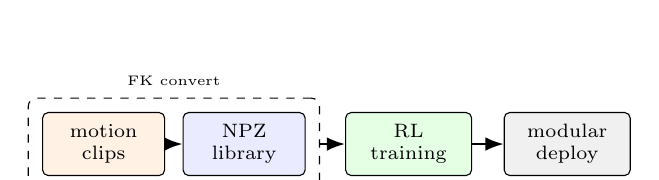
\begin{tikzpicture}[
    font=\scriptsize,
    box/.style={draw, rounded corners=2pt, align=center, inner sep=4pt,
      minimum height=0.8cm},
    group/.style={draw, dashed, rounded corners=3pt, inner sep=5pt},
    arr/.style={-{Latex}, thick},
  ]
    \node[box, fill=orange!10, minimum width=1.55cm] (clips) {motion\\clips};
    \node[box, fill=blue!8, right=0.22cm of clips, minimum width=1.55cm] (npz)
      {NPZ\\library};
    \node[group, fit=(clips)(npz)] (prep) {};
    \node[font=\tiny, anchor=south] at ([yshift=1pt]prep.north) {FK convert};
    \draw[arr] (clips) -- (npz);

    \node[box, fill=green!10, minimum width=1.6cm, right=0.5cm of npz] (train)
      {RL\\training};
    \draw[arr] (prep.east) -- (train.west);

    \node[box, fill=gray!12, minimum width=1.6cm, right=0.4cm of train] (deploy)
      {modular\\deploy};
    \draw[arr] (train) -- (deploy);
  \end{tikzpicture}
  \vspace{0.4em}
  \caption{Workflow overview (three stages). Conversion is a preprocessing step;
  training and deploy stay decoupled.}
  \label{fig:pipeline}
\end{figure}

\subsection{Motion conversion}
Source clips (CSV, PKL, or similar) are batch-converted through GPU forward
kinematics into a multi-trajectory NPZ library: frame rate, joint angles, and
per-link world-frame poses and velocities---the fields the motion command loads.
Optional motion-bundle caching speeds repeated train and play sessions.
Extension robots register conversion metadata for the same pipeline; a small
sample library ships in-tree for smoke tests while full datasets remain local
or on Hugging Face.

\subsection{Training and export}
Training and play share one CLI surface. Each run can emit policy weights and
companion metadata so external simulators and hardware stacks can load the
trained controller without importing the trainer---supporting modular deploy
rather than a monolithic sim-to-real stack. Play mode disables training-only
aids (observation corruption, assistive wrench, external pushes). A reference
G1 runtime in the companion \texttt{wbc-g1-deploy} repository
(\url{https://github.com/wbc-mjlab/wbc-g1-deploy}) shows how exported artifacts
plug into sensing, reference streaming, and actuation; the browser demo at
\url{https://wbc-mjlab.github.io/wbc-demo/} offers the same split for quick
replay without local sim or hardware.

\subsection{Validation workflow}
\label{sec:validation}
Quantitative benchmarks across presets are ongoing (Section~\ref{sec:limitations}).
Today we recommend a reproducible smoke path: convert bundled sample clips,
train or play with the target preset, and validate tracking in sim before
hardware trials.

\subsection{Robot extensions}
\label{sec:extensions}
\textsc{wbc-mjlab} is robot-agnostic at the MDP layer: rewards, RSI, motion
command, and presets do not hard-code a skeleton. To train WBC on a new
humanoid, publish a small extension package rather than forking \texttt{env/}.
The in-tree G1 stack is the template; the published H2 extension~\citep{wbc_h2_ext}
(\url{https://github.com/wbc-mjlab/wbc-mjlab-extension-h2}) shows the intended
layout end to end.

\paragraph{What an extension provides.}
\begin{enumerate}[leftmargin=1.4em,itemsep=0.12em]
  \item \textbf{Robot entity} --- MuJoCo model, anchor and keybody names, joint
        PD and action scales, contact/IMU sensors.
  \item \textbf{Task builder} --- \texttt{make\_base\_wbc\_env\_cfg()} plus a
        preset stack (typically \texttt{apply\_wbc}, optionally
        \texttt{apply\_se\_actor}) with that robot's body tuples.
  \item \textbf{Registration} --- one call to \texttt{register\_wbc\_extension}
        wires the robot id, motion-conversion metadata, project-local
        \texttt{data/<robot>/} paths, and \texttt{--task} entries into the
        same CLIs as G1 (\texttt{data-to-npz}, \texttt{train}, \texttt{play},
        \texttt{list-envs}).
\end{enumerate}
The H2 package follows this pattern: \texttt{h2\_base\_cfg()} attaches the H2
entity, \texttt{h2\_wbc\_env\_cfg()} applies the default WBC preset with H2
end-effector and keybody lists, and \texttt{Wbc-H2} registers a single task.
Install the extension editable alongside core; no changes to the shared tracker
are required.

\paragraph{Typical workflow for a new robot.}
\begin{enumerate}[leftmargin=1.4em,itemsep=0.12em]
  \item Scaffold a package with an \texttt{mjlab.tasks} entry point (mirror the
        H2 repo structure).
  \item Implement \texttt{<robot>\_base\_cfg()} and motion FK metadata for
        \texttt{wbc-mjlab-data-to-npz}.
  \item Stack an existing preset on the base config and register one default
        task id.
  \item Convert clips, train with \texttt{--task}, validate in play, then hand
        exported artifacts to a platform-specific deploy runtime.
\end{enumerate}
Paper-specific presets (ZEST repro, binary-failure RSI, SE actor) compose the
same way on any registered robot once body names and scales are set.

% ===========================================================================
\section{Positioning}
\label{sec:related}
% ===========================================================================

\textsc{wbc-mjlab} implements the low-level tracker shared by recent whole-body
systems, not their higher-level planners. Table~\ref{tab:lineage} summarizes
lineage; method papers remain the citations for scientific claims about a given
recipe. Teleoperation, multimodal planners, and teacher-distillation
stacks~\citep{clot2026,m3imic2026,handoff2026} consume the exported policy
rather than forking the MDP.

\begin{table}[t]
  \centering
  \small
  \setlength{\tabcolsep}{3.5pt}
  \caption{Lineage of ideas available as configuration on the shared template.}
  \label{tab:lineage}
  \begin{tabular}{@{}p{2.5cm}p{5.2cm}p{4.4cm}@{}}
    \toprule
    Source & In \textsc{wbc-mjlab} & Out of scope \\
    \midrule
    DeepMimic~\citep{peng2018deepmimic} & reference-state resets
      & full character stack \\
    mjlab tracking~\citep{zakka2026mjlab} & bundled command observation
      & modular reference catalog \\
    BeyondMimic & binary-failure RSI; light regularizers
      & latent diffusion; anchor-relative frames \\
    ZEST & Table~S4 ($\kappa{=}1/4$); reward-aligned EMA;
      assistive wrench & full actuator/PLA stack \\
    SONIC / OmniXtreme & body-velocity terms; obs.\ corruption; torque soft limit
      & foundation-scale / flow-matching training \\
    Deploy practice & modular ref.\ observations; SE actor; exported artifacts
      & estimators and hardware drivers \\
    \bottomrule
  \end{tabular}
\end{table}

Open WBC codebases~\citep{hybridrobotics_wbt,nvlabs_groot_wbc2026} inform the
design; \textsc{wbc-mjlab} targets a smaller,
robot-agnostic training surface on mjlab.

% ===========================================================================
\section{Limitations and Roadmap}
\label{sec:limitations}
% ===========================================================================

Coverage of prior methods is intentionally partial. BeyondMimic support centers
on RSI strategy and reward weights; anchor-relative body frames and the
diffusion stack are not implemented. SONIC-scale data and training recipes are
planned as presets rather than new MDPs.

Retargeting quality and fully robot-agnostic deploy/demo runtimes remain active
work. Global anchor tracking rewards are not yet axis-selective (e.g.\ disabling
yaw or horizontal position for SE-oriented stacks); policies trained with full
global terms may not match partial observability on hardware.
Quantitative benchmarks across presets and robots---including SE versus
non-SE actors under matched estimator noise---are left for a future revision
(Section~\ref{sec:validation}).

% ===========================================================================
\section{Acknowledgments}
% ===========================================================================

\textsc{wbc-mjlab} builds on mjlab~\citep{zakka2026mjlab}.
Design inspiration includes open Isaac Lab whole-body tracking stacks and
NVIDIA GR00T Whole-Body Control~\citep{hybridrobotics_wbt,nvlabs_groot_wbc2026}.
Please cite method papers when comparing against or reproducing their setups,
in addition to this report and mjlab. We thank the Institute of Artificial
Intelligence (MIPT), Robotics Center SBER, Innopolis University, and KAIST
for hosting and hardware used in training and deploy experiments.

\bibliographystyle{plainnat}
\bibliography{references}

\end{document}
